\chapter{Vurdering} \label{sec:vurdering}
Følgende afsnit vil vurdere på resultaterne af de to komprimeringsmetoder ved komprimering af Lena og argumentere for, hvilken af de to metoder der fungerer bedst til komprimering af mobilbilleder. Parametrene, der vil blive sammenlignet, over er billedkvalitet og komprimeringsgrad. Der vil først blive opstillet tre par bestående af hhv. et DCT-komprimeret billede og et PCA-komprimeret billede. Parrene er sammensat ved enten at have samme komprimeringsgrad eller samme SNR-værdi. Konklusionerne heraf bruges til vurdering af seks testbilleder af forskellige motiver taget med en mobiltelefon. Det ønskes her at danne en mere generel konklusion af metodernes nytte.\\
Efterfølgende vil fordele og ulemper ved de to metoder blive fremhævet, hvilke fejlkilder de er behæftet, såvel som forslag til forbedring af metoderne brugt i rapporten.

\section{Sammenligning - Lena}
Der vil i dette afsnit blive set på tre par af hhv. et DCT- og PCA-komprimeret billede. Det første par er DCT-komprimeret med Q90 og PCA-komprimeret med PC50. Dette par er sammensat på baggrund af nærliggende komprimeringsgrader, hvorved deres billedekvalitet vil blive sammenlignet. Næste par, bestående af Q50 og PC75, er sammensat grundet nærliggende SNR-værdier, der udtrykker en stor lighed i kvaliteten af billedet, hvorved komprimeringsgraden er interessant i disse par. Det sidste par har både samme komprimeringsgrad og SNR-værdi og består af Q10 og PC25.\\
Kvaliteten af billederne vurderes både objektivt og subjektivt for at påpege forskelle på den matematiske vurdering og den visuelle/subjektive vurdering, der unægtelig er nødvendig, når der undersøges billeder.

\begin{table}[htbp]
\centering
\begin{tabular}{|l|ll|ll|ll|} \hline
                    & \multicolumn{1}{l|}{\textbf{Q90}} & \textbf{PC50}   &  \multicolumn{1}{l|}{\textbf{Q50}} & \textbf{PC75}   & \multicolumn{1}{l|}{\textbf{Q10}} & \textbf{PC25}   \\ \hline
\textbf{Komprimeringsgrad}   & \textbf{1:3,79}  & \textbf{1:3,92} & 1:5,98                   & 1:3,39 & \textbf{1:7,31}                   & \textbf{1:7,44} \\ 
\textbf{\% ændret pixel}     & 89,38                    & 94,02  & 92,78                    & 92,65  & 96,16                    & 95,53  \\ \hline
\textbf{Gns. ændring}        & 2,96                     & 6,12   & 4,51                     & 4,79   & 8,49                     & 8,66   \\
\textbf{Gns. ændring (R)}   & 2,39                     & 5,25   & 3,71                     & 3,89   & 7,95                     & 7,95   \\
\textbf{Gns. ændring (G)}  & 2,99                     & 6,85   & 4,62                     & 5,28   & 8,79                     & 9,84   \\
\textbf{Gns. ændring (B)}   & 3,51                     & 6,26  & 5,21                     & 4,79   & 8,73                     & 8,19   \\ \hline
\textbf{Max ændring (R)}   & 22                       & 59     & 48                       & 45     & 110                      & 87     \\
\textbf{Max ændring (G)}  & 39                       & 96     & 62                       & 62     & 124                      & 130    \\
\textbf{Max ændring (B)}   & 43                       & 88     & 87                       & 81     & 110                      & 105    \\ \hline
\textbf{SNR}                 & 292,41                   & 53,04  & \textbf{106,58}                   & \textbf{95,39}  & \textbf{29,77}                    & \textbf{23,68}  \\ \hline
\end{tabular}
\caption{Komprimeringsdata i sammenligningespar (fed indikerer sammenligningsparametre)}
\label{tb:sammenligning}
\end{table}

%\multicolumn{1}{l|}{Q75} & PC100  &
%1:5,12                   & 1:2,05 &
%91,67                    & 91,66  &
%3,77                     & 3,93   &
%3,03                     & 3,10   &
%3,82                     & 4,24   &
%4,47                     & 4,48   &
%33                       & 36     &
%55                       & 44     &
%70                       & 63     &
%161,64                   & 155,38 &


\subsection*{Q90 og PC50 - komprimering}
Komprimering med Q90 og PC50 har ca. samme komprimeringsgrad, hvorved de nedbringer det originale billede til ca. samme filstørrelse. Dette betyder, at kvaliteten af billederne kan sammenlignes og i dette specifikke komprimeringstilfælde konkluderes på, hvilken af metoderne, der giver bedste kvalitet. Ses der på SNR-værdierne i tabel \ref{tb:SNR_DCT} og \vref{tb:SNR_PCA}, bliver det tydeligt, at DCT leverer en betydelig  bedre billedkvalitet end PCA. Dette fremkommer af en SNR, der er ca. seks gange så stor som for PCA. Dette understøttes yderligere af den gennemsnitlige ændring i pixelværdierne, hvor PCA har over dobbelt så stor en ændring. Store pixelændringer giver specielt store udslag i SNR, hvilket ses ved, at PCA-komprimeringen har betydeligt større maksimale ændringer end DCT. Der kan i ovenstående sammenligning konkluderes, at rent matematisk leverer DCT en bedre billedekvalitet end PCA ved samme komprimeringsgrad.

\subsubsection{Subjektiv vurdering Q90 og PC50}
Rent subjektivt kan der ved sammenligning af Q90 og PC50, ses en stor forskel på billederne. Ved Q90 er det for det menneskelige øje ikke muligt at se en forskel fra det originale, og kvaliteten synes derfor uændret. Ved PC50 ses det til gengæld, at der er sket en markant ændring i billedet - billedet synes grumset. Dette skyldes ændringer i mange pixels i hele billedet. Fejlbillederne i figur \ref{fig:noiseQ90} og \ref{fig:noisePC50} bekræfter dette - for Q90 ses næsten ingen fejl, da billedet er nær konstant gråt, mens der for PC50 ses tydelige ændringer i det grå billede.\\
De subjektive og objektive vurderinger stemmer altså overens, da Q90 producerer et billede, som både objektivt og subjektivt er af højere kvalitet end billedet produceret med PC50.

%\subsection*{Q75 + PCA100 - SNR}
%Komprimering med Q75 og 100 principale komponenter resulterer i lignende SNR ($161.64 \approx 155.38$) efter komprimering. SNR-værdierne underbygges af de maksimale pixelændringer, der er tæt på ens og ellers ligeligt fordelt mellem de to metoder. Den gennemsnitlige pixelændring i de forskellige farver illustrerer ydermere den ensformige komprimering meget godt ved, at de for DCT er lidt større end for PCA. Dette resulterer også i en lidt højere gennemsnitlig ændring på tværs af alle farverummene, men dette er også afspejlet i SNR-værdien.
%Undersøges komprimeringsgraden fremkommer det at DCT komprimerer ca. dobbelt så meget som PCA i dette tilfælde. Altså leverer DCT en komprimeret fil halv så stor som PCA gør, men med samme billedkvalitet. Dette taler for brug af DCT ved disse komprimeringsgrader.
%
%De to billeder har samme SNR, hvilket indikerer lige stor mængde støj i begge billeder i forhold til det originale billede. Det ses imidlertid, at PCA100 er af langt ringere kvalitet end Q75 – billedet fremstår grumset hvorimod Q75 fremstår næsten lige så klart for det menneskelige øje, som det originale billede. Undersøges fejlbillederne for de to billeder er det også tydeligt at se, at PCA100 har langt tydeligere fejl end Q75. Fejlbilledet for Q75 viser at det komprimerede billede har små fejl alle steder i billedet, hvor der er store kontraster, mens fejlbilledet for PCA100 har fejl spredt over hele billedet. Disse er mere tydelige, og dette gør, at PCA100 fremstår som værende af ringere kvalitet end Q75 trods samme SNR som Q75. Ydermere er billedet behandlet med Q75 komprimeret i højere grad – næsten dobbelt så meget.
%De subjektive og objektive vurderinger stemmer altså ikke overens. Trods lignende SNR'er viser det sig, at komprimering med 100 principale komponenter producerer et billede, som for det menneskelige øje, er af væsentligt ringere kvalitet end bileddet komprimeret ved Q75.

\subsection*{Q50 og PC75 - SNR}
Komprimering med Q50 og PC75 resulterer i en tilnærmelsesvist lignende SNR-værdi ($106,58 \approx 95,39$) efter komprimering.\\
Når SNR for de to billeder er relativt ens, kan komprimeringsgraden sammenlignes, og det fremkommer her, at Q50 komprimerer næsten dobbelt så meget som PC75. Det vurderes, at Q50 leverer samme billedkvalitet som PC75 men ved højere komprimeringsgrad.

\subsubsection{Subjektiv vurdering af Q50 og PC75}
Ved Q50 kan det ses, at billedet er komprimeret - DCT har skabt blokke af pixels, som ikke er korrelerede, og dette kan ses i det færdige billede. Det fremgår ligeledes af fejlbilledet i figur \ref{fig:noiseQ50}, at der er fejl langs alle kanter, som består af bratte farveskift.\\
Ved billedet med PC75 er uskarpt og grumset. Det ses desuden der ved fejlbilledet, at der er lavet markante ændringer i hele billedet. Fejlbilledet ses i figur \ref{fig:noisePC75}.
Trods de lignende SNR'er synes billedet lavet ved Q50 at være af højere kvalitet end billedet lavet ved PC75, dog er forskellen ikke nær så stor som ved Q90 og PC50.

\subsection*{Q10 og PC25 - SNR og komprimering}
Q10 og PC25 er valgt på baggrund af den objektive kvalitet i form af deres SNR-værdier og samtidig en næsten ens komprimeringsgrad. Med Q10 ses det, at SNR ligger en anelse højere end PC25 på trods af at den gennemsnitlige afvigelse af pixels, som er lavere med Q10. Grunden til en større afvigelse på trods af en højere SNR-værdi ved Q10, er metoden ved beregning af SNR, hvor der fremkommer tal i anden potens. Dvs., at hvis eksemplvis blå optræder med enkelte meget høje tal ved Q10, og med PC25 lavere tal flere gange, vil de høje tal have enorm stor betydning. Derfor kan der opstå højere procentvis ændring af pixels og samtidig højere SNR-værdi ved samme metode. \\
Det vurderes at ved høje komprimeringsgrader, laver metoderne billeder af tilnærmelsesvis ens kvalitet.

\subsubsection{Subjektiv vurdering af Q10 og PC25}
På begge billeder ses det tydeligt, at der er foregået en høj komprimering og dermed en forringelse af kvaliteten. DCT har lavet blokke af korrelerede pixels, men som ikke er korrelerede blokke imellem - dette ses som tydelige firkantede elementer i billedet. Billedet med 25 principale komponenter er meget utydeligt og grumset i en sådan grad, at Lenas ansigtsudtryk har ændret sig betragteligt. Fejlbillederne i figur \ref{fig:noiseQ10} og \ref{fig:noisePC25} bakker det op ved meget tydelige ændringer for PC25, som kommer til udtryk som meget mørke og lyse områder i disse. Komprimeringen ved Q10 må siges at give et bedre billedkvalitetsmæssigt resultat ved den subjektive vurdering.

\begin{figure}
\begin{minipage}[b]{0.31\linewidth}
\centering
\includegraphics[width=0.8\textwidth]{Billeder/fejlbilleder/fejl10.png}
\caption{\href{https://www.dropbox.com/home/P1\%20-\%20B205/vejleder/billeder/DCT/Fejlbilleder?preview=fejl10.png}{Støj ved Q10}}
\label{fig:noiseQ10}
\end{minipage}
\hspace{0.2cm}
\begin{minipage}[b]{0.31\linewidth}
\centering
\includegraphics[width=0.8\textwidth]{Billeder/fejlbilleder/fejl50.png}
\caption{\href{https://www.dropbox.com/home/P1\%20-\%20B205/vejleder/billeder/DCT/Fejlbilleder?preview=fejl50.png}{Støj ved Q50}}
\label{fig:noiseQ50}
\end{minipage}
\hspace{0.2cm}
\begin{minipage}[b]{0.31\linewidth}
\centering
\includegraphics[width=0.8\textwidth]{Billeder/fejlbilleder/fejl90.png}
\caption{\href{https://www.dropbox.com/home/P1\%20-\%20B205/vejleder/billeder/DCT/Fejlbilleder?preview=fejl90.png}{Støj ved Q90}}
\label{fig:noiseQ90}
\end{minipage}
\hspace{0.2cm}
\end{figure}
\begin{figure}
\begin{minipage}[b]{0.31\linewidth}
\centering
\includegraphics[width=0.8\textwidth]{Billeder/fejlbilleder/fejlPC25.png}
\caption{\href{https://www.dropbox.com/home/P1\%20-\%20B205/vejleder/billeder/PCA/Fejlbilleder?preview=fejlPC25.png}{Støj ved PC25}}
\label{fig:noisePC25}
\end{minipage}
\hspace{0.2cm}
\begin{minipage}[b]{0.31\linewidth}
\centering
\includegraphics[width=0.8\textwidth]{Billeder/fejlbilleder/fejlPC50.png}
\caption{\href{https://www.dropbox.com/home/P1\%20-\%20B205/vejleder/billeder/PCA/Fejlbilleder?preview=fejlPC50.png}{Støj ved PC50}}
\label{fig:noisePC50}
\end{minipage}
\hspace{0.2cm}
\begin{minipage}[b]{0.31\linewidth}
\centering
\includegraphics[width=0.8\textwidth]{Billeder/fejlbilleder/fejlPC75.png}
\caption{\href{https://www.dropbox.com/home/P1\%20-\%20B205/vejleder/billeder/PCA/Fejlbilleder?preview=fejlPC75.png}{Støj ved PC75}}
\label{fig:noisePC75}
\end{minipage}
\end{figure}

\subsection*{Delkonklusion - Lena}
En konklusion på sammenligningen af DCT og PCA på Lena kan overvejende udtrykkes som, at begge metoder leverer omtrent samme SNR-værdi, dvs. objektivt samme billedkvalitet, såvel som lignende komprimeringsgrader ved lave komprimeringskvaliteter. Dog er DCT bedre til at komprimere ved høje komprimeringskvaliteter, og samtidig holde en bedre billedkvalitet end PCA. På trods af at PCA er god til at komprimere billedet ved få principale komponenter, ses det tydeligt, at den har svært ved at komprimere særlig meget, når et vis antal principale komponenter gør sig gældende. Det er klart, da billedet ændrer sig mindre og mindre jo flere principale komponenter, der bruges. På trods af at DCT også komprimerer bedre ved lave kvaliteter, er der flere "komprimeringsgrader" \ ved PCA, da der ved Lena er alt fra PC1 til PC512 at benytte sig af, hvorimod DCT kun har Q1 til Q100. Altså er spændet af komprimeringsgrader for PCA større end for DCT.\\
Hvordan dimensionerne af billedet påvirker resultatet i forhold til komprimeringsmetoden undersøges som det næste. Til sidst vil alle observationer fra Lena blive be- eller afkræftet ved en test af større billeder taget med en mobiltelefon.

\subsection{Skalering af Lena}
Det er interessant at kigge på, hvordan både DCT og PCA opfører sig ved forskellige størrelser af Lena. Ved at skalere billedet ned til halv størrelse, fra $512 \times 512$ pixels til $256 \times 256$ pixels, har billedet samme struktur men færre dimensioner. Dette kan udnyttes til at se på, om parametre som komprimeringsgraden og SNR-værdien ændrer sig drastisk ved størrelsesændring. For at dokumentere sammenhænge tilstrækkeligt, er fem forskellige kvantiseringsgrader og fem forskellige antal principale komponenter benyttet. Jævnfør figur \ref{fig:SkaleringLena-Komprimering}, ses det at komprimeringen ved både DCT og PCA forholder sig nogenlunde ens. Udsvingene er grundet i, at det samme billede skal repræsenteres ved færre pixels. Dette betyder, at komprimeringen ved det mindre $256 \times 256$ billede nødvendigvis må afvige lidt fra det større $512 \times 512$ billede. Denne observation bekræfter os i, at størrelsen af billedet ikke har den store betydning hvad komprimeringsgraden angår - dvs. at effektiviteten forbliver den samme. \\
Jævnfør figur \ref{fig:SkaleringLena-SNR} ses igen nogle tendenser. På trods af at DCT overvejende har samme tendens, har det mindre billede væsentligt lavere SNR-værdier ved Q25, Q50 og Q75. Lignende ses det ved PCA, da det mindre billede har væsentligt lavere SNR-værdier ved alle komprimeringer udover PC25 end det større. I begge tilfælde kan det tyde på, at antal pixels betyder en del for SNR-udregningen. Endvidere observeres en ensartethed ved både PCA og DCT ved det større billede, hvor de fungerer ens. \\
Tendensen for både komprimerings- og SNR-graferne er, at begge metoder fungerer respektivt ens ved mindre og større billeder, dog med mindre udsving.

\begin{figure}[htbp]
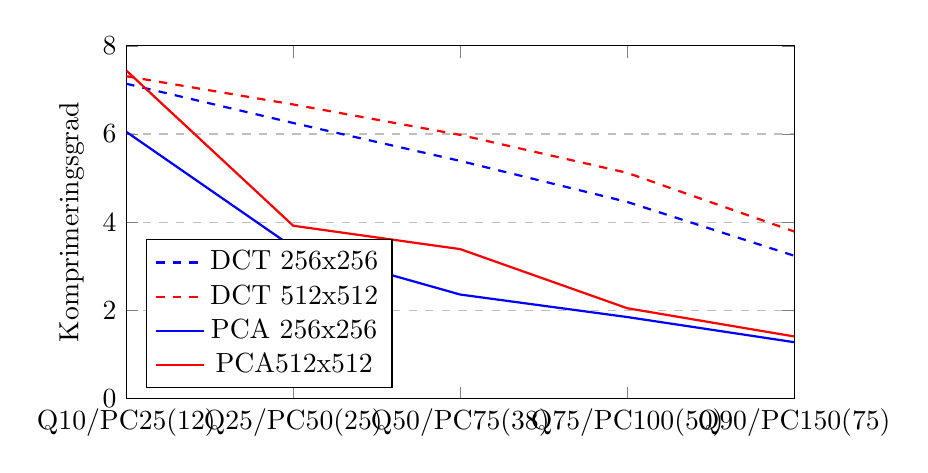
\begin{tikzpicture}
\begin{axis}[
%    title={Komprimering af skaleret billede},
    xlabel={},
    ylabel={Komprimeringsgrad},
    width = 0.83*\textwidth,
    height = 0.5*\textwidth,
    xtick = {0,1,2,3,4},
    xmin=0, xmax=4,
    ymin=0, ymax=8,
    %x tick label style = {anchor = east},
    xticklabels={Q10/PC25(12),Q25/PC50(25),Q50/PC75(38),Q75/PC100(50),Q90/PC150(75)},
    ytick={},
    legend pos=south west,
%    legend style={
%                at={(0,0)}},
    ymajorgrids=true,
    grid style=dashed,
]
 
\addplot[
    color=blue,
    dashed,
    thick,
    ]
    coordinates {
    (0,7.14)(1,6.25)(2,5.39)(3,4.46)(4,3.24)
    };
\addplot[
    color=red,
    dashed,
    thick,
    ]
    coordinates {
    (0,7.31)(1,6.67)(2,5.98)(3,5.12)(4,3.79)
    };
\addplot[
    color=blue,
    thick,
    ]
    coordinates {
    (0,6.05)(1,3.43)(2,2.36)(3,1.85)(4,1.28)
    };
\addplot[
    color=red,
    thick,
    ]
    coordinates {
    (0,7.44)(1,3.92)(2,3.39)(3,2.05)(4,1.41)
    };
]
\legend{DCT 256x256,DCT 512x512, PCA 256x256, PCA512x512}
\end {axis}
\end{tikzpicture}
\caption{Komprimeringsgrad for DCT og PCA ved skaleret Lena}
\label{fig:SkaleringLena-Komprimering}
\end{figure}

\begin{figure}[htbp]
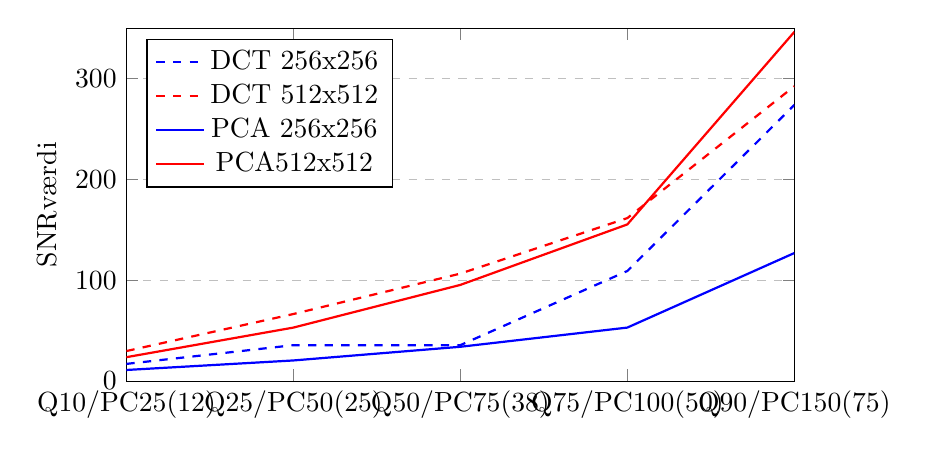
\begin{tikzpicture}
\begin{axis}[
%    title={SNR-værdier af skaleret billede},
    xlabel={},
    ylabel={SNRværdi},
    width = 0.83*\textwidth,
    height = 0.5*\textwidth,
    xtick = {0,1,2,3,4},
    xmin=0, xmax=4,
    ymin=0, ymax=350,
    xticklabels={Q10/PC25(12),Q25/PC50(25),Q50/PC75(38),Q75/PC100(50),Q90/PC150(75)},
%    x tick label style={rotate=45},
    ytick={},
    legend pos=north west,
%    legend style={
%                at={(0,0)}},
    ymajorgrids=true,
    grid style=dashed,
]
 
\addplot[
    color=blue,
    dashed,
    thick,
    ]
    coordinates {
    (0,17.02)(1,35.60)(2,35.61)(3,109.19)(4,273.85)
    };
\addplot[
    color=red,
    dashed,
    thick,
    ]
    coordinates {
    (0,29.77)(1,66.51)(2,106.58)(3,161.64)(4,292.41)
    };
\addplot[
    color=blue,
    thick,
    ]
    coordinates {
    (0,10.99)(1,20.44)(2,34.01)(3,53.05)(4,126.98)
    };
\addplot[
    color=red,
    thick,
    ]
    coordinates {
    (0,23.68)(1,53.04)(2,95.39)(3,155.38)(4,346.31)
    };
]
\legend{DCT 256x256,DCT 512x512, PCA 256x256, PCA512x512}
\end{axis}
\end{tikzpicture}
\caption{SNR-værdier for DCT og PCA ved skaleret Lena}
\label{fig:SkaleringLena-SNR}
\end{figure}

\section{Vurdering af mobilbilleder}
%Intro til afsnit
%Hvorfor giver mobilbilleder mening
%Hvilke præmisser er der (ny størrelse, billede, osv.)
%Hvordan komprimereres de (hvilke PCA og Q), hvorfor
%Resultater (hvorfor ingen gennemsnit osv.)
%Bekræfter ovenstående test, vores konklusion på baggrund af lena?
Det forsøges, at generalisere konklusionen fra foregående afsnit, der i sin essens lød, at de to komprimeringsmetoder var lige gode ved lave komprimeringskvaliteter, mens DCT var betydeligt bedre ved højere kvaliteter. For at kunne generalisere denne konklusion vil seks forskellige billeder blive taget med en mobiltelefon (noteret som T1, T2, …, T6), og vist i figur \ref{fig:T1} til \ref{fig:T6}. Disse billeder vil blive komprimeret med de to metoder, og ved hhv. en lav, mellem og høj komprimeringskvalitet for at sammenligne resultaterne.

\begin{figure}[!h]
\begin{minipage}[b]{0.3\linewidth}
\centering
\includegraphics[width=\textwidth]{Billeder/test_billeder/T1.jpg}
\caption{\href{https://www.dropbox.com/home/P1\%20-\%20B205/vejleder/billeder/Mobilbilleder/T1?preview=T1.jpg}{Mobilbillede \phantom{m} T1}}
\label{fig:T1}
\end{minipage}
\hspace{0.5cm}
\begin{minipage}[b]{0.3\linewidth}
\centering
\includegraphics[width=\textwidth]{Billeder/test_billeder/T2.jpg}
\caption{\href{https://www.dropbox.com/home/P1\%20-\%20B205/vejleder/billeder/Mobilbilleder/T2?preview=T2.jpg}{Mobilbillede T2}}
\label{fig:T2}
\end{minipage}
\hspace{0.5cm}
\begin{minipage}[b]{0.3\linewidth}
\centering
\includegraphics[width=\textwidth]{Billeder/test_billeder/T3.jpg}
\caption{\href{https://www.dropbox.com/home/P1\%20-\%20B205/vejleder/billeder/Mobilbilleder/T3?preview=T3.jpg}{Mobilbillede T3}}
\label{fig:T3}
\end{minipage}
\end{figure}

\begin{figure}[!h]
\begin{minipage}[b]{0.3\linewidth}
\centering
\includegraphics[width=\textwidth]{Billeder/test_billeder/T4.jpg}
\caption{\href{https://www.dropbox.com/home/P1\%20-\%20B205/vejleder/billeder/Mobilbilleder/T4?preview=T4.jpg}{Mobilbillede T4}}
\label{fig:T4}
\end{minipage}
\hspace{0.5cm}
\begin{minipage}[b]{0.3\linewidth}
\centering
\includegraphics[width=\textwidth]{Billeder/test_billeder/T5.jpg}
\caption{\href{https://www.dropbox.com/home/P1\%20-\%20B205/vejleder/billeder/Mobilbilleder/T5?preview=T5.jpg}{Mobilbillede T5}}
\label{fig:T5}
\end{minipage}
\hspace{0.5cm}
\begin{minipage}[b]{0.3\linewidth}
\centering
\includegraphics[width=\textwidth]{Billeder/test_billeder/T6.jpg}
\caption{\href{https://www.dropbox.com/home/P1\%20-\%20B205/vejleder/billeder/Mobilbilleder/T6?preview=T6.jpg}{Mobilbillede T6}}
\label{fig:T6}
\end{minipage}
\end{figure}

Billederne er taget i en opløsning på $2448 \times 3264$ pixels, hvilket er væsentligt større end Lena med dimensionerne $512 \times 512$ pixels. De specifikke komprimeringskvaliteter for DCT og PCA er valgt ud fra resultaterne med Lena.\\
Der er valgt tre par af komprimeringer, der udtrykker hhv. en lav, mellem og høj komprimeringskvalitet. Disse er bestemt til at være Q10, Q50 og Q90. PC25, PC75 og PC150 har tilnærmelsesvis samme SNR som disse ved komprimering af Lena, så disse vælges på baggrund af dette. Da mobilbillederne, som der undersøges med herunder, er langt større, skaleres antallet af principale komponenter op, så det passer til størrelsen af billederne. Dette betyder, at parrene kommer til se således ud
\begin{itemize}
	\item[]{Q10 og PC120}
	\item[]{Q50 og PC360}
	\item[]{Q90 og PC720}
\end{itemize}
For hvert af parrene sammenlignes SNR og komprimeringsgrad. I figur \ref{fig:mobilbilleder_SNR} ses grafer for SNR for  begge metoder med alle billederne. På samme måde illustrerer figur \ref{fig:mobilbilleder_komprimering} grafer for komprimeringsgraderne. Desuden er der inkluderet en graf for komprimering af Lena udført med Q10, Q50, Q90 og PC25, PC75 og PC150 for sammenligning.
\definecolor{dblue}{HTML}{0000CC}
%\definecolor{lblue}{HTML}{6666FF}
\definecolor{dgreen}{HTML}{006600}
%\definecolor{lgreen}{HTML}{329932}
\definecolor{dred}{HTML}{CC0000}
%\definecolor{lred}{HTML}{FF6666}
\definecolor{dturquoise}{HTML}{2C9C91}
%\definecolor{lturquoise}{HTML}{79E9DE}
\definecolor{dpurple}{HTML}{660066}
%\definecolor{lpurple}{HTML}{A64CA6}
\definecolor{dorange}{HTML}{CC8400}
%\definecolor{lorange}{HTML}{FFB732}
\begin{figure}
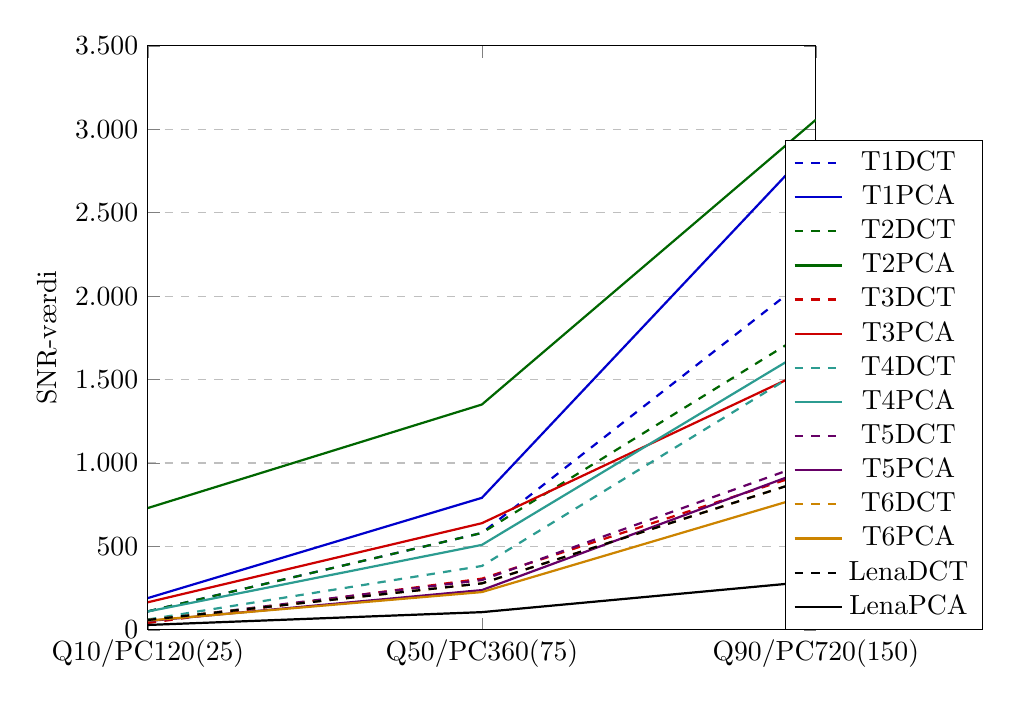
\begin{tikzpicture}
\begin{axis}[
%    title={SNR-værdi ved komprimering af mobilbilleder},
    xlabel={},
    ylabel={SNR-værdi},
    width = 0.83*\textwidth,
    height = 9cm,
    xtick = {0,1,2},
    xmin=0, xmax=2,
    ymin=0, ymax=3500,
    y tick label style={
        /pgf/number format/.cd,
       		use comma,
        	/tikz/.cd},
    %x tick label style = {anchor = east},
    xticklabels={Q10/PC120(25),Q50/PC360(75),Q90/PC720(150)},
    ytick={},
    legend pos=south east,
    legend style={
                at={(1.25,0)}},
    ymajorgrids=true,
    grid style=dashed,
]
 
\addplot[
    color=dblue,
    dashed,
    thick,
    ]
    coordinates {
    (0,111.36)(1,581.01)(2,2145.30)
    };
\addplot[
    color=dblue,
    thick,
    ]
    coordinates {
    (0,190.95)(1,791.52)(2,2914.51)
    };
\addplot[
    color=dgreen,
    dashed,
    thick,
    ]
    coordinates {
    (0,111.36)(1,581.01)(2,1817.41)
    };
\addplot[
    color=dgreen,
    thick,
    ]
    coordinates {
    (0,730.56)(1,1350.62)(2,3056.68)
    };
\addplot[
    color=dred,
    dashed,
    thick,
    ]
    coordinates {
    (0,41.72)(1,307.30)(2,958.41)
    };
\addplot[
    color=dred,
    thick,
    ]
    coordinates {
    (0,165.83)(1,639.55)(2,1581.68)
    };
\addplot[
    color=dturquoise,
    dashed,
    thick,
    ]
    coordinates {
    (0,62.54)(1,383.17)(2,1608.79)
    };
\addplot[
    color=dturquoise,
    thick,
    ]
    coordinates {
    (0,110.57)(1,509.59)(2,1712.87)
    };
\addplot[
    color=dpurple,
    dashed,
    thick,
    ]
    coordinates {
    (0,56.44)(1,298.69)(2,1016.79)
    };
\addplot[
    color=dpurple,
    thick,
    ]
    coordinates {
    (0,53.10)(1,238.69)(2,978.65)
    };
\addplot[
    color=dorange,
    dashed,
    thick,
    ]
    coordinates {
    (0,59.80)(1,279.01)(2,918.94)
    };
\addplot[
    color=dorange,
    thick,
    ]
    coordinates {
    (0,55.94)(1,226.80)(2,819.59)
    };
    \addplot[
    color=black,
    dashed,
    thick,
    ]
    coordinates {
    (0,59.80)(1,279.01)(2,918.94)
    };
\addplot[
    color=black,
    thick,
    ]
    coordinates {
    (0,29.77)(1,106.58)(2,292.41)
    };
	\legend{T1DCT, T1PCA, T2DCT, T2PCA, T3DCT, T3PCA, T4DCT, T4PCA, T5DCT, T5PCA, T6DCT, T6PCA, LenaDCT, LenaPCA}
\end{axis}
\end{tikzpicture}
\caption{SNR-værdier for mobilbilleder}
\label{fig:mobilbilleder_SNR}
\end{figure}

\begin{figure}
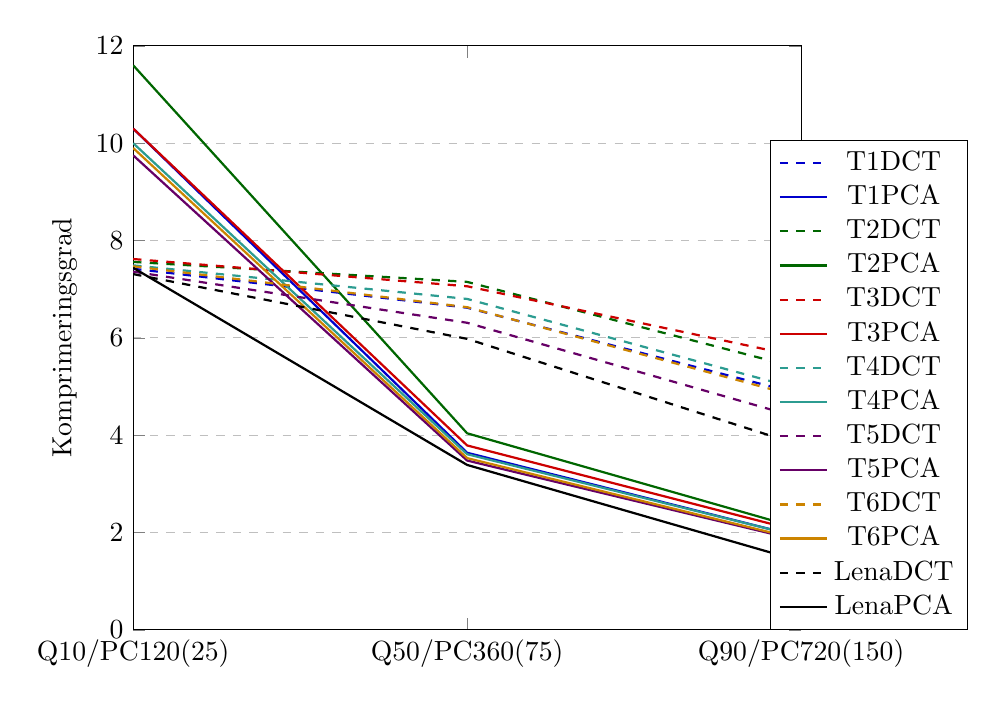
\begin{tikzpicture}
\begin{axis}[
%    title={Komprimeringsgrad af mobilbilleder},
    xlabel={},
    ylabel={Komprimeringsgrad},
    width = 0.83*\textwidth,
    height= 9cm,
    xtick = {0,1,2},
    xmin=0, xmax=2,
    ymin=0, ymax=12,
    %x tick label style = {anchor = east},
    xticklabels={Q10/PC120(25),Q50/PC360(75),Q90/PC720(150)},
    ytick={},
    legend pos=south east,
    legend style={
                at={(1.25,0)}},
    ymajorgrids=true,
    grid style=dashed,
]
 
\addplot[
    color=dblue,
    dashed,
    thick,
    ]
    coordinates {
    (0,7.42)(1,6.62)(2,4.84)
    };
\addplot[
    color=dblue,
    thick,
    ]
    coordinates {
    (0,10.30)(1,3.64)(2,1.91)
    };
\addplot[
    color=dgreen,
    dashed,
    thick,
    ]
    coordinates {
    (0,7.56)(1,7.15)(2,5.37)
    };
\addplot[
    color=dgreen,
    thick,
    ]
    coordinates {
    (0,11.60)(1,4.04)(2,2.08)
    };
\addplot[
    color=dred,
    dashed,
    thick,
    ]
    coordinates {
    (0,7.62)(1,7.06)(2,5.61)
    };
\addplot[
    color=dred,
    thick,
    ]
    coordinates {
    (0,10.30)(1,3.79)(2,2.02)
    };
\addplot[
    color=dturquoise,
    dashed,
    thick,
    ]
    coordinates {
    (0,7.49)(1,6.80)(2,4.94)
    };
\addplot[
    color=dturquoise,
    thick,
    ]
    coordinates {
    (0,10.00)(1,3.61)(2,1.91)
    };
\addplot[
    color=dpurple,
    dashed,
    thick,
    ]
    coordinates {
    (0,7.36)(1,6.31)(2,4.35)
    };
\addplot[
    color=dpurple,
    thick,
    ]
    coordinates {
    (0,9.75)(1,3.48)(2,1.83)
    };
\addplot[
    color=dorange,
    dashed,
    thick,
    ]
    coordinates {
    (0,7.47)(1,6.63)(2,4.78)
    };
\addplot[
    color=dorange,
    thick,
    ]
    coordinates {
    (0,9.90)(1,3.53)(2,1.85)
    };
   	    \addplot[
    color=black,
    dashed,
    thick,
    ]
    coordinates {
    (0,7.31)(1,5.98)(2,3.79)
    };
\addplot[
    color=black,
    thick,
    ]
    coordinates {
    (0,7.44)(1,3.39)(2,1.41)
    };
	\legend{T1DCT, T1PCA, T2DCT, T2PCA, T3DCT, T3PCA, T4DCT, T4PCA, T5DCT, T5PCA, T6DCT, T6PCA, LenaDCT, LenaPCA}
\end{axis}
\end{tikzpicture}
\caption{Komprimgeringsgrad af mobilbilleder}
\label{fig:mobilbilleder_komprimering}
\end{figure}

\subsubsection{Q10 og PC120}
Det ses af grafen i figur \ref{fig:mobilbilleder_SNR}, at PC120 opnår højere SNR for billede T1, T2 og T3, end DCT gør. Dette skyldes formentlig, at disse billeder indeholder få bratte ændringer - de består af mange glatte overgange, og PCA kan derfor let udtrykke meget af billedet ved få principale komponenter. DCT med Q10 opnår mindre støj i T5 og T6, hvilket er en følge af, at der er flere forskellige farver i disse billeder. For T4 opnås ca. samme SNR for de to metoder.
Det ses desuden på grafen i figur \ref{fig:mobilbilleder_komprimering}, at PC120 tilmed opnår en højere komprimeringsgrad end DCT ved Q10.\\
På papiret er PC120 bedre end Q10, men i praksis bruges disse komprimeringsgrader sjældent, da de laver billeder af en uønskværdig kvalitet.

\subsubsection{Q50 og PC360}
Det ses af grafen i figur \ref{fig:mobilbilleder_SNR}, at PCA ved PC360 stadig opnår bedre SNR end DCT med Q50 for billede T1, T2 og T3. Resultaterne for sammenligningen af SNR er tilmed magen til dem for Q10 og PC120 for de resterende billeder. Det ses dog på grafen i figur \ref{fig:mobilbilleder_komprimering}, at Q50 opnår væsentligt bedre komprimering end PC360 for alle seks billeder.

\subsubsection{Q90 og PC720}
Sammenligningen af Q90 og PC720 har samme grundlæggende tendenser som den ovenstående - PCA giver for T1, T2 og T3 bedre billedkvalitet end DCT, mens DCT håndterer T5 og T6 bedre. De opnår lignende resultater for T4. DCT opnår dog imidlertid langt højere komprimeringsgrad end PCA gør og billederne fylder dermed mindre, hvilket er ønskværdigt.\\
Bemærk, at DCT opnår både bedre SNR og komprimeringsgrad for alle par ved komprimering af Lena.

\subsubsection{Delkonklusion - mobilbilleder}
Komprimering af mobilbillederne giver anderledes resultater, end komprimering af Lena gør. Ikke desto mindre opnår PCA stadig ringere komprimering end DCT ved højere kvaliteter. Dette ses dog i lyset at, at PCA opnår bedre SNR. PCA håndterer altså mobilbillederne bedre end den håndterer Lena.\\
At PCA er bedre ved lave kvaliteter er nær ubrugeligt, da det ikke er interessant at se på ringe kvaliteter - dette er derfor en negligerbar egenskab. DCT indgår et mere ønskværdigt kompromis med kvaliteten for højere komprimeringsgrad - mobilbilleder skal komprimeres meget og bibeholde kvaliteten. DCT må derfor siges at være bedre end PCA til komprimering af mobilbilleder.

%Det fremkommer i disse resultater at PCA gennemgående er bedre til at komprimere ved den lave kvalitet. Her giver PCA bedre SNR-værdi, såvel som højere komprimeringsgrad. Dette skyldes at PCA bruger de første få komponenter til at udtrykke en stor del af billedet, hvorved det meget hurtigt kan skabe en tilnærmelse af billedet, og de resterende komponenter udtrykker "blot" \ detaljer i billedet, der ikke har stor betydning for det samlede resultat. Derudover komprimerer PCA meget godt, når den kun bruger få komponenter. Dette ses også i tabel \ref{tb:komprimering_PCA1} og \vref{tb:komprimering_PCA2}. Det skal dog bemærkes, at der ved T2 og T3 er betydeligt bedre SNR-værdier med PCA end DCT, hvilket skyldes den store ensformighed i billederne, hvilket gør at PCA fungerer bedre.\\
%Når kvaliteten øges til mellem kvalitet ($Q50$ og $PCA360$), ses der gennemgående et udsving i resultaterne, hvor komprimeringsgraden for PCA falder betydeligt i forhold til DCT. Ligesom med Lena er det gennemgående, at DCT holder en nogenlunde stabil komprimeringsgrad på tværs af kvaliteterne, hvor PCA har et større udsving i komprimeringsgraden. Dette illustrerer figur \ref{fig:mobilbilleder_komprimering} også, hvor den generelle hældning for PCA-komprimeringerne er højere end for DCT.\\
%Undersøges resultaterne ved den høje komprimeringskvalitet ($Q90$ og $PCA720$) bliver det igen tydeligt, at der er forskel på billederne der arbejdes med. PCA-komprimeringerne af T2 og T3 giver betydeligt bedre SNR-værdier end DCT, men har også betragteligt lavere komprimeringsgrader. Dette skyldes at T2 og T3 er meget ensformige, og ved en høj kvalitet har PCA nok principale komponenter til at repræsentere detaljer og derved forbedre SNR-værdien. Da DCT ikke tilpasser sig dataene den transformerer, vil denne ikke være i stand til i samme grad at tage højde for den store ensformighed.\\
%I modsætning til Lena-billedet ved forholdsvist mange principale komponenter og en kvantiseringstabel på $Q90$, ses det at ved T4, T5 og T6 ligger SNR-værdierne tæt på hinanden. Det kan skyldes den enorme forskellighed i billedet, hvor PCA og DCT i og for sig udligner hinanden ved styrker og svagheder forskellige steder på billedet. Det fremgår dog klart at DCT stadig er langt mere effektiv til at komprimere ved høj billedkvalitet.
%Endvidere hvis resultaterne vurderes subjektivt, ses det ligesom den objektive vurdering, at PCA fungerer bedre ved ensformige billeder, da den ikke behøver mange principale komponenter for at udtrykke hele billedet - T2 er et glimrende eksempel på dette. Modsat et meget kontrastfyldt billede, dvs. med mange ændringer, skal PCA bruge enormt mange principale komponenter for at udtrykke små ændringer i billedet. I dette tilfælde vil DCT give bedre resultater, da den blot udglatter de små ændringer - T6 kunne være et eksempel på dette. \fxnote{Lineær komprimeringsgrad for PCA - skal flettes ind i teksten på et tidspunkt}

\section{Fejlkilder}
I forbindelse med brug af hhv. DCT og PCA til komprimering af billeder er der nogle begrænsninger og fejlkilder, som påvirker resultatet. Det følgende afsnit vil præsentere disse fejlkilder, såvel som den indflydelse de har på resultaterne.

\subsubsection{DCT fejlkilder}
Den diskrete cosinustransformation fungerer i billedkomprimeringsalgoritmer, fordi den energikomprimerer et signal effektivt. Dette er imidlertid kun tilfældet, når signalet er glat. Når der snakkes om billeder, vil det sige, at farveintensiteter i alle $8 \times 8$ matricer er relativt ens, eller udtrykker en glat overgang. Hvis billedet ikke har denne egenskab, skal transformationen bruge mange cosinusfunktioner til at udtrykke billedet, og der vil ikke blive opnået en god energikomprimering. Er der derfor mange bratte ændringer i billedet, vil det resultere i at DCT ikke vil være i stand til at komprimere så godt. \\
Netop fordi at DCT bygger på cosinustransformationer, der er svingninger, har denne metode også problemer med at udtrykke bratte ændringer korrekt. Med de 64 cosinusfunktioner (se ligning \vref{eq:DCTeq}, hvor $n=8$), der bruges i denne transformation (hvoraf dem med højeste frekvens ofte fjernes i kvantiseringen og afrundingen), er det ikke muligt at repræsentere bratte ændringer godt. Dette resulterer i at der omkring kanter, hvor der er stor ændring, typisk opstår større fejl og unøjagtigheder end i andre dele af billedet.

DCT fungerer på $8 \times 8$ matricer, men såfremt et billedes dimensioner ikke kan divideres med otte, vil den sidste matrix ikke indeholde tilstrækkelige data til at udfylde alle indgange. Der er to mulige løsninger til problemet: ikke at komprimere den yderste kant (op til syv pixels) af billedet eller at nulfylde kanten, så billeddimensionerne går op i otte [\citet{zero_padding}, s. 1]. Komprimeres kanten ikke vil det give en dårligere komprimeringsgrad, da tallene ikke vil blive centreret omkring nul, og Huffmankodningen vil derfor ikke fungere optimalt i disse kanter. Nulfyldes kanten, hvilket svarer til at lave en grå kant, vil der i mange billeder opstå en brat ændring mellem billedet og kanten, hvilket vil have betydning for komprimeringen af kanten, såvel som at det dekomprimerede billede vil være påvirket af den grå kant jævnfør tidligere fejlkilder.
%En alternativ løsning kunne være at fylde de resterende pixels med en spejling af de yderste pixels. Dette vil betyde at den tilføjede kant ligner de pixels der ligger ud til kanten. Dette kan dog give fejl, hvis de pixels der spejles ud i kanten repræsenterer en brat kontrast. Dette vil resultere i at kontrasten fremgår to gange. I mange tilfælde, må det dog kunne forventes at kunne give et bedre resultat end en nulfyldning.

\subsubsection{PCA fejlkilder}
PCA bruges normalt til reducering af dimensioner på store datasæt og for at finde sammenhænge, der ikke nødvendigvis er tydelige, når der kigges på dataene. PCA reducerer herved dimensionerne til de mest betydende, og derved kan store dimensioner af data nedbringes til få betydende dimensioner. Det er ikke helt samme præmis, der er i spil, når PCA bliver brugt som billedekomprimeringsmetode. Her er der ikke nødvendigvis samme sammenhæng mellem de enkelte rækker af pixels, som der er mellem målinger i et datasæt, som PCA normalvis bruges på. Dette betyder, at PCA fungerer godt til at reducere dimensionerne meget, men dette resulterer ikke nødvendigvis i gode resultater visuelt. Det betyder også, at når PCA ikke reducerer dimensionerne meget, men bibeholder en betydelig mængde principale komponenter, så ændrer kvaliteten sig ikke meget, men komprimeringsgraden falder. PCA er altså ikke beregnet til billedkomprimering, men kan med acceptable resultater bruges til det.

Når det komprimerede billede gemmes til en fil, opstår der en fejlkilde. For at få sammenlignelige data bruges Huffmankodning også på PCA, men for at denne metode giver mening, skal tallene, der gemmes, være heltal. Dette er problematisk, da egenvektorerne i $P$ er ortonormale, hvorved alle indgange er meget små for tilsammen at give en længde på én. Dette gør, at en afrunding fuldstændigt eliminerer nærmest samtlige værdier i $P$. Ved at multiplicere alle indgangene med 10.000 inden de afrundes og Huffmankodes, opnåes heltal på op til fire cifre. Tallene divideres blot med 10.000 i dekodningen, og afrundingen, der før ændrede alle indgange til nul, afrunder nu blot på det, der svarer til femte decimal. Dette ændrer på dataene, der i dekomprimeringen ikke bliver de eksakt samme, men der kan ses bort fra fejlene fremkommet ved denne afrunding, da disse anses som ubetydeligt små.

\subsubsection{Generelle fejlkilder}
Når de komprimerede billeder dekomprimeres, sker det, at de dekomprimerede pixelværdier afviger fra de tilladte værdier $0 \leq \text{pixelværdi} \leq 255$. Dette skyldes afrundingen af tallene i forbindelse med, at filerne bliver gemt med Huffmankodning. Dette betyder imidlertid, at alle tal under nul trunkeres til at være nul og alle tal over 255 til 255. Dette er dog i meget få tilfælde nødvendigt og er typisk tal, der i forvejen ville være endt på 255. Der vil altså ikke være en visuel tydelig forskel ved denne ændring.

Den subjektive vurdering af billedkvalitet er netop subjektiv, og det kan ikke regnes med, at denne siger noget endegyldigt om komprimeringsteknikkerne, med mindre det bakkes op af statistiske beviser i form af store datasæt fra store empiriske undersøgelser.
I denne rapport er det kun gruppemedlemmerne, der har vurderet subjektivt på billederne, derfor kan der ikke siges at være statistisk belæg for konklusionerne, hvorved de blot bør anses som bemærkninger/suppleringer til den objektive vurdering.

I forbindelse med generaliseringen af delkonklusionen, der er udformet på baggrund af resultater med komprimering af Lena, sammensættes par af Q-værdier og antal principale komponenter, for at have ensformige data at vurdere på ved mobilbillederne. Disse par er dog sammensat på baggrund af metodernes effektivitet på Lena og ved andre billeder, kan disse par vise sig at være misvisende og ikke give udtryk for samme kvalitet, som de oprindeligt var udvalgt til. Denne pardannelse antages at give et nogenlunde grundlag for sammenligning.